\documentclass[journal]{new-aiaa}
%\documentclass[conf]{new-aiaa} for conference papers
\usepackage[utf8]{inputenc}

\usepackage{graphicx}
\usepackage{amsmath}
\usepackage[version=4]{mhchem}
\usepackage{siunitx}
\usepackage{longtable,tabularx}
\setlength\LTleft{0pt} 
\usepackage{float}

\title{Evolution of the Transient Mach Disk}

\author{Brodie J. Norfolk \footnote{Student, Department of Mechanical, Aerospace, and Mechatronics Engineering, Building 31, Monash University, Victoria 3800 , and AIAA Student Member.}}
\affil{Laboratory for Turbulence Research in Aerospace and Combustion, Monash University, Australia}


\begin{document}

\maketitle

\begin{abstract}
Here we present a shock structure tracking technique and detailed discussion on the fluid dynamics of transient supersonic jets. We explore the fundamental fluid dynamics of transient supersonic jets with variation of the exit flow nozzle geometry and plate impingement. Our nozzle geometries include a convergent, divergent, and convergent-divergent design. The impingement of transient supersonic jets has previously been studied, however it is absent of extensive data, high quality schlieren, and variable exit geometry. We aim to address absences in the literature, explore in detail the shock-vortex interaction during jet impingement, and track the progression of the shock structure with a novel algorithm. Our discussion of the fundamental fluid dynamics governing the transient supersonic jet process details the affects of alternating the incident Mach number for, nozzle geometry variation on the shock-vortex interaction and jet plate impingement.
% These instructions give you guidelines for preparing papers for AIAA Technical Journals using \LaTeX{}. If you previously prepared an AIAA Conference Paper using the Papers Template, you may submit using the Papers Template so long as the text is double-spaced.  Carefully follow the journal paper submission process in Sec.~II of this document. Keep in mind that the electronic file you submit will be formatted further at AIAA. This first paragraph is formatted in the abstract style. Abstracts are required for regular, full-length papers and express articles. Be sure to define all symbols used in the abstract, and do not cite references in this section. The footnote on the first page should list the Job Title and AIAA Member Grade (if applicable) for each author.
\end{abstract}

\section*{Nomenclature}

{\renewcommand\arraystretch{1.0}
\noindent\begin{longtable*}{@{}l @{\quad=\quad} l@{}}
$M_1$ &  ambient Mach number\\
$P_1$ &  ambient pressure, Pa\\
$P_4$ &  shock tube driver section pressure, Pa\\
$U_1$ &  ambient air velocity, m/s\\
$U_4$ &  shock tube driver section air velocity, m/s\\
$\gamma_1$ &  ambient specific heat ratio\\ 
$\gamma_4$ &  ambient specific heat ratio\\
\multicolumn{2}{@{}l}{Subscripts}


\end{longtable*}}




\section{Introduction}
%\lettrine{T}{his} document is a \LaTeX{} template for preparation of papers for AIAA Technical Journals. If you are reading a hard-copy or .pdf version of this document, download the electronic file, new-aiaa.cls, and use it to prepare your manuscript.
%
%Authors using \url{https://www.overleaf.com} may simply open the AIAA template from the Overleaf gallery to work online; no local installation of any files is required. Authors using a local \LaTeX{} installation will need to open the template in Overleaf and use the ``Download as zip'' option from the project menu to download a local copy of the template files. To create your formatted manuscript, type your own text over sections of the template, or cut and paste from another document and then use the available markup styles. Note that special formatting such as subscripts, superscripts, and italics may be lost when you copy your text into the template from a Word Processing program such as Microsoft Word. See Sec. IV for more detailed formatting guidelines.

Gas turbine engines are an integral component for the function of ground based power generation and aircraft engines. They account for a large percentage of power generation world wide. Thermodynamic cycle advances in gas turbine design play an important role in preventing the growth of emissions pollution and prolonged global warming \cite{paxson2018pressure}. Pressure gain combustion (PGC) is one possible to method of efficiency improvement. PGC is a constant volume combustion process that operates by increasing the stagnation pressure entering the turbine via heat released from combustion. Increasing the turbine inlet pressure allows for considerably more work to be extracted when the turbine expands the flow back to the free stream pressure. PGC optimises gas turbine thermodynamic cycle efficiency, and has the potential to increase current engine efficiency up to 10\% \cite{gulen2013constant}.

PGC is at peak efficiency when accomplished through detonation driven combustion, this involves the implementation of detonation waves within the combuster to cause an increase in the temperature and pressure of the fuel-air mixture \cite{eidelman1991review}. During combustion, detonation waves produce flow at supersonic velocities leading to an approximate constant volume and significant pressure gain across the combustor. For supersonic velocities high pressure turbine inlet flow must be steady. A possible method to achieve steady flow at the turbine inlet is via the implementation of a pulse detonation engine \cite{kailasanath2009research} with an equalising plenum chamber. Wear on the first stage of the turbine presents itself as one of the most significant problems of PGC implemetation in current engines. Replacing the combustor in a conventional gas turbine with a pulse detonation combustor (PDC) will result in the propergating detonation waves to converge on the first stage of the turbine. This overtime can lead to concentrated wear on the first stage of the turbine high wear stress points \cite{dean2005operation}. To alleviate turbine wear, the utilization of a high pressure plenum chamber is placed at the exit of the PDC, and creates steady flow conditions effectively shielding the first stage of the turbine from combustion detonations. It remains unclear on how to integrate a pressure plenum into a PDC design. 

The fluid dynamics characterising the governing flow at the exit of PDC is defined as a shock-driven, transient, supersonic jet process \cite{radulescu2007transient}. The governing flow can be classified into several different stages \cite{ishii1999experimental} as shown in Figure \ref{fig:0}. The first stage of jet evolution is defined by the diffraction of a shock wave around the corners of the tube exit, this region is bounded by the curved part of the incident shock, the nozzle lip, and a reflected sound wave. 
%\begin{figure}[h]  
%\centering
%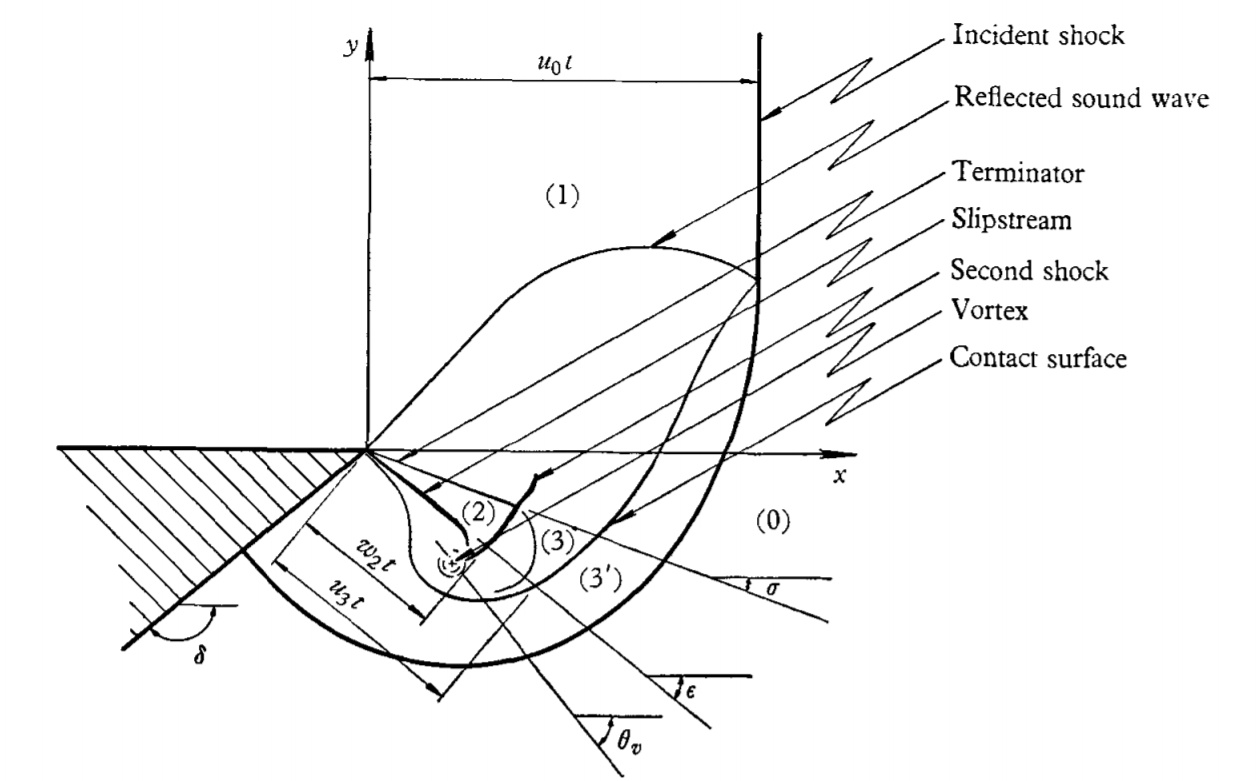
\includegraphics[scale=0.7]{fig0.PNG}
%\caption{Features of the diffraction pattern \cite{skews1967}}
%\label{fig:0}
%\end{figure}
In the next stage of jet evolution, a vortex ring is generated by the roll-up of the shear layer due to Kelvin-Helmholtz type instabilities along the slipstream at the nozzle lip \cite{elder1952experimental,dora2014role}. Kelvin-Helmholtz instabilities exist within the shock as a result of external perturbations (inhomogeneities in the flow) producing oscillations in the vortex sheet separating fluids with different flow characteristics. This structure propagates down the jet axis, and is simultaneously accompanied by the translation of a curved barrel shock formed initially at the nozzle lip. This instigates the formation of a curved Mach disk for a ratio of the nozzle exit to free-stream pressure exceeding $2.06$ \cite{matsuda1987numerical}. MORE ON MACH DISK

A triple point occurs between the leading edge of the barrel shock, the second shock, and the Mach disk. Given a sufficiently strong jet, a slip surface is generated downstream of the triple point. The first shock cell is formed in the third stage of jet evolution which is marked by the pinch-off phenomenon of the vortex ring, and signals the start of the trailing jet phase \cite{gharib1998universal}. Separation of the vortex ring from the flow structure is driven by Kelvin-Helmholtz instabilities within the shear layer of the trailing jet \cite{zhao2000effects}. The final stage of the supersonic jet is defined by the point at which the transient jet and vortex are no longer joined and the trailing jet forms. This is accompanied by the formation of a quasi-steady shock cell in self-sustained oscillation, radiating strong pressure waves. %These four stages of jet evolution are illustrated in Figure \ref{fig:2}.
%\begin{figure}[h] 
%	\centering
%	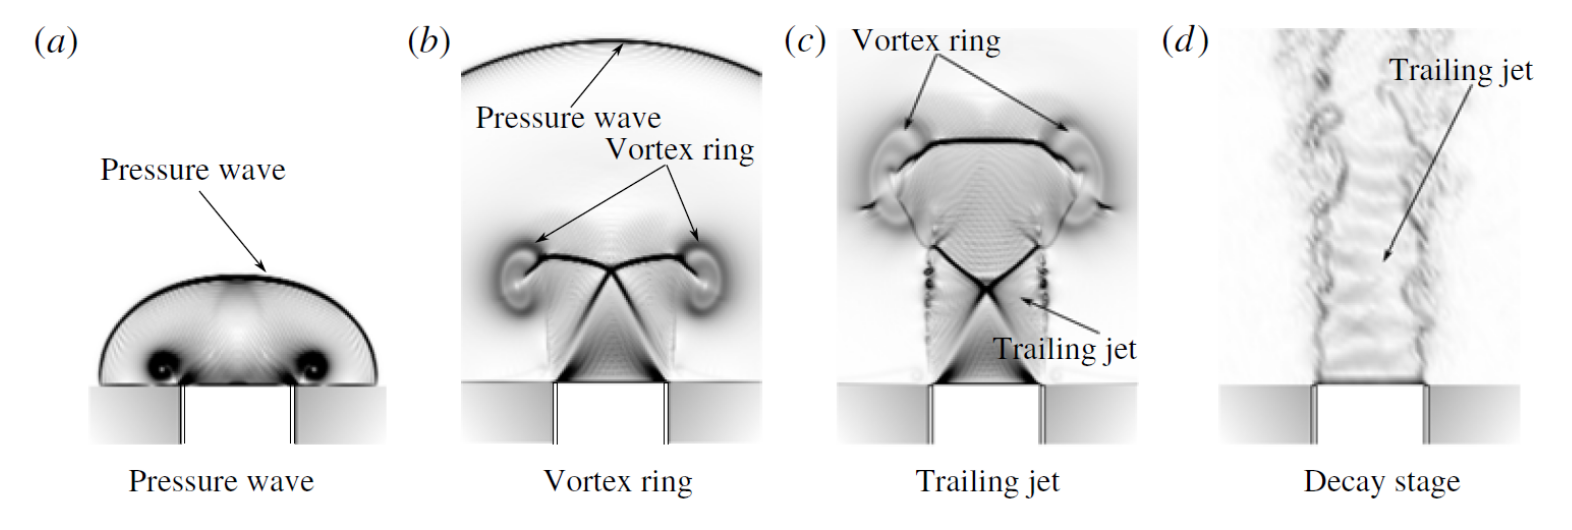
\includegraphics[scale=0.28]{fig2.png} 
%	\caption{Evolution of the transient supersonic jet. (a) Diffracting shock/Pressure
%		wave. (b) Axial translation of the vortex rings, formation of the curved shock and an unsteady Mach disk. (c) Formation of the trailing supersonic jet. (d) Decay of the trailing jet and the end of the transient jet
%		process. \cite{fernández2017}}
%	\label{fig:2}
%\end{figure}

Investigation into the high pressure plenum chamber required for PDEs currently has not been undertaken. However, the flow dynamics is considered analogous to the impingement of a transient supersonic jet on a flat plate. The governing dynamics of transient jet impingment can be classified into serveral stages as The physical process is initially characterised by the reflection of the incident shock wave on the impinging plate. The reflected shock wave propargates back towards the nozzle and interacts with the approaching vortex ring. The central section of the reflected shock wave is captured by the embedded rearward-facing shock at the centre of the vortex ring, and is intensified by the opposing high-speed flow. Simultaneously, the outer section of the shock wave is diffracted by the vortex core. This process results in the formation of a toroidal shock wave which focuses in the trailing jet along the longitudinal axis of flow. The next stage of the fluid dynamics is defined by the impingement of the propagating vortex ring. Initially, as the vortex ring approaches the wall, its propagation velocity decreases and its diameter increases due to the adverse pressure gradient present \cite{szumowski2000starting}. After votex impingement the vortical flow undergoes rapid radial expansion developing a boundary layer on the surface, which slows down the flow and increases the pressure distribution over the plate. After a given duration that is dependent on the initial incident Mach number, the boundary layer separates from the plate and the flow rolls up generating a series of secondary vortices. This also occurs at the thin shear layer present between the jet flow and the exterior fluid as the region rolls up due to Kelvin-Helmholtz instabilities. This produces small interacting secondary vortex rings that propagate towards the plate \cite{minota1997shock}. Cumulative interactions between the primary and secondary wall vortex rings result in a near standing lift off of the pair. The secondary ring subsequently merges with the primary ring, and the weakened newly formed vortex ring continues to translate down the plate. %Stages of impingement are illustrated in Figure \ref{fig:4} below.

%\begin{figure}[h] 
%	\centering
%	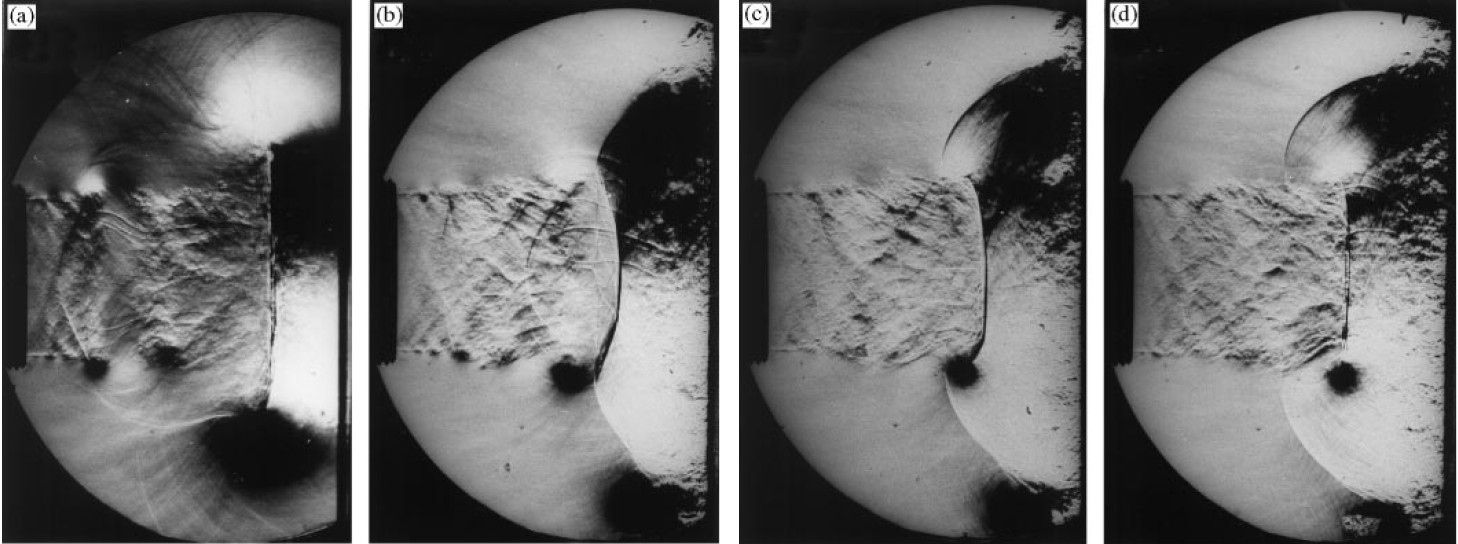
\includegraphics[scale=0.9]{fig4.PNG} 
%	\caption{Evolution of jet impingement. (a) Impingement of vortex ring. (b) Vortex ring translates down the plate. (c) Secondary vortex formation. (d) Lift-off of votex rings and dissapation. \cite{szumowski2000}}
%	\label{fig:4}
%\end{figure}
%For a plate of variable angle, the lower core of the vortex ring impinges initially, and generates an asymmetric set of secondary vortices. These new flow structures orbit around the main vortex, creating a temporarily thicker boundary layer at the lower end of the flow field. Again after a period of time, dependent on the incident Mach number, he boundary layer separates from the plate. This results in the vortex ring pivoting on the lower core, undergoing negligible deformation, towards the surface plate. The upper core then impinges on the plate and the upper wall vortex is generated. This new structure begins to expand radially increasing in thickness due to the remaining jet flow. While simultaneously, the lower wall vortex propagates around the outer limits of the main vortex, stops expanding, and dissipates into a  thin structure. The impinging jet continues to feed into the upper section of the flow field, generating  wall vortices with a thicker upper core. For lower angles of plate alignment, the flow field shows an increase in overall velocity, and visible curvature of the vortex ring structure during impingement. The toroidal shock wave that forms as a result of impingement propagates perpendicularly with respect to the surface \cite{mariani2013}.  
%
%The far-field noise developed by the shock wave-vortex interaction can be decomposed into three components, the sound field due to the formation and evolution of the vortex ring, the reflection shock and vortex ring interaction noise production, and the noise due to impingement of the ring on the plate. The plate-votex ring impingement noise is produced by fluctuating pressure due to the deformation and stretching of the vortex ring, formation and growth of a secondary wall vortex ring, and lifting-off of the primary-secondary vortex ring pair \cite{murugan2010}.

\section{Experimental Methods}
\subsection{Shock Tube Facility}
The experiments presented were conducted in the LTRAC Supersonic Jet Facility. A schematic of the facility is shown in Figure \ref{shocktube}. 

The facility utilises compressed air delivered by the Monash University compressed air supply system. To produce a canonical transient supersonic jet a shock tube model is adopted \cite{john1962shock}. A typical shock tube consists of a high pressure section (driver section) and a low pressure section (driven section) separated by a diaphragm. Air enters the driver section until a desired pressure is reached, the diaphragm is then ruptured via a puncture from an actuated pin. Following the rupture, compression waves are fired down the driven section by the high pressure gas in the driver. As these compression waves travel down the tube they coalesce and form a shock wave that propagates into the test section, diffracts, and produces a transient supersonic jet. The shock tube model is fitted with a converging nozzle and impinging plate, shown in Figure \ref{attachment}. 

To prevent reflecting flow and acoustic feedback loop interference, the converging nozzle was designed with a $60^\circ$ exterior angle and a $0.5mm$ lip. During the evolution of a transient supersonic jet, the vortex is fully formed at approximately 3 inner diameters from the exit for a conventional, no nozzle, shock tube \cite{mariani2013head}. As a result, an impingement plate distance is chosen DISTANCE AND WHY. The plate diameter is designed to appear infinite to the flow.

ENTER SHOCK TUBE FIGURE AND NOZZLE/PLATE FIGURE
ENTER TABLE WITH DIMENSIONS

The relationship between the driver (4) pressure ratio and the ambient (1) pressure of the system is shown in Equation \ref{shock}, and was utilised to calculate the design incident Mach number propagating from the shock tube \cite{anderson2010fundamentals}.

\begin{equation} \label{shock}
\frac{P_4}{P_1} = \frac{2\gamma_1M_1^2 - (\gamma_1 - 1)}{\gamma_1 + 1}\left(1 - \frac{\gamma_{4-1}}{\gamma_{1+1}}\frac{U_1}{U_4}\left(M_1 - \frac{1}{M_1}\right)\right)^{-2\gamma_4/\gamma_{4-1}}
\end{equation}

\subsection{Schlieren Imaging}
The shock-driven, transient, supersonic jet is measured using a Toepler Z-type schlieren apparatus \cite{settles2001schlieren} (illustrated in Figure \ref{fig:3}) with the Shimadzu HPV-1 camera. The Shimadzu has a resolution of 312 x 260 pixels and a frame rate of up to 1 million fps. 

ENTER SCHLIEREN SKEMATIC

\subsection{Post Processing}
Schlieren imaging produces a path integrated density gradient image that is excellent for flow visualisation but, is difficult to quantitatively extract physical parameters directly from image data. 
the required second order image derivatives are computed by convolution with the second order derivatives of the Gaussian kernel (reference). Mathematically this means that if f denotes the image and G the normalised Gaussian, we compute
EQUATIONS
where * denotes spatial convolution, x=(x,y) denotes the pixel position, and the derivative directions i and j can be x or y. The eigenvectors and eigenvalues are computed in the algorithm from a standard second derivative Hessian matrix 

HESSIAN MATRIX
Use a normalised ranking to threshold intensity lower then the 90th percentile 

\section{Results and Discussion}
\subsection{Converging Nozzle}
\subsection{Impinging Plate}
\subsection{Mach Number Variation}
\subsection{Convergence Study}
%\section{Procedure for Paper Submission}
%
%All manuscripts are to be submitted online at \url{https://mc.manuscriptcentral.com/aiaa}. Select either “Log In” if you have an existing account or “Create an Account” if this is your first time submitting to one of AIAA’s journals. If it’s the latter, please follow the instructions ScholarOne provides. Once you have logged into ScholarOne, select “Author Center” then scroll down. Under “Author Resources”, select the star beside “Click here to submit a new manuscript”. The site will take you step-by-step through the submission process. Once you submit your manuscript, you will receive an email containing your manuscript ID number as well as a link to view the status of your manuscript. 
%
%After entering all required submission data, you must use the “Upload Manuscript” feature of the Author Center to upload your submission. Remember that your document must be in single-column, double-spaced format (as this template) before you upload it. Please be sure that the name of the file you upload for processing is short and simple (i.e., “SmithJPP.pdf”) with no spaces, tildes, symbols, or other special characters. Authors are encouraged to upload .pdf files, which are less likely to have conversion errors on upload. Failure to meet these requirements could result in a processing error that would require you to re-upload your manuscript. Once you have uploaded your manuscript, please inspect the file for accuracy. This step is required to complete your submission. If you experience difficulties with the upload and/or conversion of your manuscript, please contact ScholarOne Manuscripts Support (\url{https://mchelp.manuscriptcentral.com/gethelpnow/} or +1-888-503-1050) for additional assistance. 
%
%\emph{Attention Asian Authors: If you are uploading a .pdf file, please remove Asian fonts from your file, under File>Properties.}
%
%\section{General Guidelines}
%
%The following section outlines general (nonformatting) guidelines to follow. These guidelines are applicable to all authors and include information on the policies and practices relevant to the publication of your manuscript.
%
%\subsection{Publication by AIAA}
%Your manuscript cannot be published by AIAA if:
%\begin{enumerate}
%\item The work is classified or has not been cleared for public release.
%\item The work contains copyright-infringing material.
%\item The work has been published or is currently under consideration for publication or presentation elsewhere. (Exception: Papers presented at AIAA conferences may be submitted to AIAA journals for possible publication.)
%\end{enumerate}
%
%You will be asked to provide the publication or presentation history of your paper (or any similar paper) if it has \emph{ever} been submitted for publication or presentation previously to an AIAA journal or conference. Please include the following, if applicable: the full name of the publication or conference, the entire paper number, dates the conference took place, review history, final disposition of manuscript, etc.
%
%
%\subsection{Copyright}
%
%Before AIAA can publish any paper, the copyright information must be completed in ScholarOne. Failure to complete the form correctly could result in your paper not being published. You must select one copyright assignment statement (select A, B, C, or D) and once a statement is picked, changes cannot be made during the proofs stage. Read the copyright statements carefully. AIAA requires a copyright transfer from the author(s) to AIAA or a license to print your material; government authors can assert that the work is in the public domain. Because you will be completing this form online, you do not need to fill out a hard-copy form. Do not include a copyright statement anywhere on your paper. The correct statement will be included automatically at the time of processing. (If your paper was presented at an AIAA conference, then the copyright statement chosen for the journal article should be the same as for your conference paper.)
%
%\subsection{Publication Charges for Open Access}
%
%Publication charges are voluntary, and nonpayment has no influence on the review process of the time from acceptance to publication. Publication charge payments help defray production costs and keep journal subscription prices low. 
%
%The article publication charge for Open Access is available in ScholarOne and on the AIAA website; the fee is the same regardless of article type. There is a fee for Open Access immediately upon publication in AIAA’s electronic library, Aerospace Research Central (ARC) and a fee for Open Access 12 months after publication in ARC.
%
%
%\section{Instructions}
%
%If you are using the AIAA Journals \LaTeX{} Template file to prepare your manuscript, you can simply type your own text over sections of this document, or cut and paste from another document and use the available markup styles. If you choose to cut and paste, select the text from your original document and choose Edit>Copy. (Do not select your title and author information, since the document spacing may be affected. It is a simple task to reenter your title and author information in the template.) Open the Journals Template. Place your cursor in the text area of the template and select Edit>Paste. Please note that special formatting (e.g., subscripts, superscripts, italics) may be lost when you copy your text into the template.
%
%To apply the AIAA Journals formatting, use the standard \LaTeX{} commands for sections and subsection, etc; all the styles you will need to format your document are available as standard \LaTeX{} commands. The style will automatically adjust your fonts and line spacing. Repeat this process to apply formatting to all elements of your paper. \emph{Do not change the font sizes, line spacing, or margins. Do not manually hyphenate your document.} Use italics for emphasis; do not underline. 
%
%Use the Print option under the File tab to view Page Layout and see the most accurate representation of how your final paper will appear. Once formatting is complete, be sure to double space all sections of your manuscript.
%
%
%\subsection{Document Text}
%The default font for the Template is Times New Roman, 10-point size. The first line of every paragraph should be indented, and all lines should be double-spaced. Default margins are 1 in. on all sides. In the electronic version of this template, all margins and other formatting are preset. There should be no additional (blank) lines between paragraphs.
%
%\emph{NOTE:} If you are using the Template to format your manuscript, the required spacing and formatting will be applied automatically.
%
%
%\subsection{Headings}
%Format the title of your paper in bold, 18-point type, with capital and lower-case letters, and center it at the top of the page. The names of the authors, business or academic affiliation, city, and state/province follow on separate lines below the title. The names of authors with the same affiliation can be listed on the same line above their collective affiliation information. Author names are centered, and affiliations are centered and in italic type. The affiliation line for each author includes that author’s city, state, and zip/postal code (or city, province, zip/postal code and country, as appropriate). The first footnote (bottom of first page) contains the job title and department name, and AIAA member grade for each author. Author email addresses may be included also.
%
%Major headings in the template (``sections'' in the \LaTeX{} template commands) are bold 11-point font and centered. Please omit section numbers before all headings unless you refer frequently to different sections. Use Roman numerals for major headings if they must be numbered.
%
%Subheadings (``subsections'' in the \LaTeX{} template commands) are bold, flush left, and either unnumbered or identified with capital letters if necessary for cross-referencing sections within the paper. There must be at least 2 of all subheadings and sub-subheadings. If there is only a single subheading or sub-subheading, please italicize the title of the subheadings, followed by a period, and run it into the text paragraph. 
%
%Sub-subheadings (``subsubsections'' in the \LaTeX{} template commands) are italic, flush left, and either unnumbered or numbered with Arabic numerals (1, 2, 3, etc.) if necessary for cross-referencing sections within the paper.
%
%
%\subsection{Abstract}
%An abstract appears at the beginning of Full-Length Papers, Regular Articles, and Express Articles. (Survey and Design Forum Papers, History of Key Technologies Papers, invited lectures, and Technical/Engineering Notes do not include abstracts.) The abstract is one paragraph (not an introduction) and complete in itself (no reference numbers). It should indicate subjects dealt with in the paper and state the objectives of the investigation. Newly observed facts and conclusions of the experiment or argument discussed in the paper must be stated in summary form; readers should not have to read the paper to understand the abstract. Format the abstract bold, indented 3 picas (1/2 in.) on each side, and separated from the rest of the document by two blank lines.
%
%
%\subsection{Nomenclature}
%Papers with many symbols may benefit from a nomenclature list that defines all symbols with units, inserted between the abstract and the introduction. If one is used, it must contain all the symbology used in the manuscript, and the definitions should not be repeated in the text. In all cases, identify the symbols used if they are not widely recognized in the profession. Define acronyms in the text, not in the nomenclature. 
%
%\subsection{Biographies}
%Survey Papers and some Full-Length Papers include author biographies. These biographies are one paragraph each and should use the abstract formatting style.
%
%\subsection{Footnotes and References}
%Footnotes, where they appear, should be placed above the 1'' margin at the bottom of the page. To insert footnotes into the template, use the Insert>Footnote feature from the main menu as necessary. Footnotes are formatted automatically in the template, but if another medium is used, should appear in superscript as symbols in the sequence, *, $\dag$, $\ddag$, \S, \P, **, $\dag\dag$, $\ddag\ddag$, \S\S, etc.
%
%List and number all references at the end of the paper. Corresponding bracketed numbers are used to cite references in the text \cite{vatistas1986reverse}, including citations that are an integral part of the sentence (e.g., ``It is shown in \cite{dornheim1996planetary} that\ldots '') or follow a mathematical expression: ``$A^{2} + B = C$ (Ref.~\cite{terster1997nasa}).'' For multiple citations, separate reference numbers with commas \cite{peyret2012computational,oates1997aerothermodynamics}, or use a dash to show a range \cite{volpe1994techniques,thompsonspacecraft,chi1993fluid}. Reference citations in the text should be in numerical order.
%
%In the reference list, give all authors' names; do not use ``et al.'' unless there are six authors or more. Papers that have not been published should be cited as ``unpublished''; papers that have been submitted or accepted for publication should be cited as ``submitted for publication.'' Private communications and personal website should appear as footnotes rather than in the reference list.
%
%References should be cited according to the standard publication reference style (for examples, see the ``References'' section of this template). Never edit titles in references to conform to AIAA style of spellings, abbreviations, etc. Names and locations of publishers should be listed; month and year should be included for reports and papers. For papers published in translation journals, please give the English citation first, followed by the original foreign language citation.
%
%\subsection{Figures and Tables}
%Insert tables and figures within your document; they may be either scattered throughout the text or grouped all together at the end of the file. Do not insert your figures in text boxes. Figures should have no background, borders, or outlines. In the \LaTeX{} template, use the ``caption'' command to type caption text. Captions are bold with a single tab (no hyphen or other character) between the figure number and figure description. See the Table 1 example for table style and column alignment. If you wish to center tables that do not fill the width of the page, simply highlight and “grab” the entire table to move it into proper position.
%
%
%\begin{table}[hbt!]
%\caption{\label{tab:table1} Transitions selected for thermometry}
%\centering
%\begin{tabular}{lcccccc}
%\hline
%& Transition& & \multicolumn{2}{c}{}\\\cline{2-2}
%Line& $\nu''$& & $J'' $& Frequency, cm$^{-1}$& $FJ$, cm$^{-1}$& $G\nu $, cm$^{-1}$\\\hline
%a& 0& P$_{12}$& 2.5& 44069.416& 73.58& 948.66\\
%b& 1& R$_{2}$& 2.5& 42229.348& 73.41& 2824.76\\
%c& 2& R$_{21}$& 805& 40562.179& 71.37& 4672.68\\
%d& 0& R$_{2}$& 23.5& 42516.527& 1045.85& 948.76\\
%\hline
%\end{tabular}
%\end{table}
%
%
%\begin{figure}[hbt!]
%\centering
%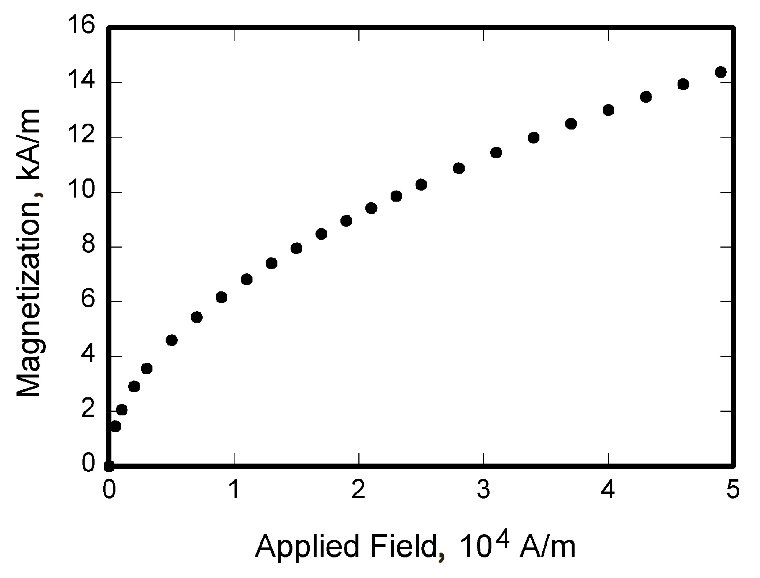
\includegraphics[width=.5\textwidth]{graph}
%\caption{Magnetization as a function of applied fields.}
%\end{figure}
%
%Line drawings must be clear and sharp. Make sure that all lines and graph points are dark and distinct and that lettering is legible; 8- to 10-point type is suitable for artwork that is sized to fit the column width (3 ¼ in.). Keep the lettering size and style uniform both within each figure and throughout all of your illustrations. Place figure captions below each figure, and limit caption length to 20-25 words. If your figure has multiple parts, include the labels “a),” “b),” etc., below and to the left of each part, above the figure caption. Please verify that the figures and tables you mention in the text actually exist. When citing a figure in the text, use the abbreviation “Fig.” except at the beginning of a sentence. Do not abbreviate “Table.” Number each different type of illustration (i.e., figures and tables) sequentially with relation to other illustrations of the same type.
%
%Figure labels must be legible after reduction to column width (preferably 8--10 points after reduction).
%
%All tables are numbered consecutively and must be cited in the text; give each table a definitive title. Be sure that you have a minimum of two columns (with headings) and two rows to constitute a proper table; otherwise reformat as a displayed list or incorporate the data into the text. Plan tables to fit the column width (3 ¼ in.) or the journal page width (7 in.). Position a double rule at the top and bottom of each table and single rule under the column headings; do not use shading, border lines, or vertical rules between table columns. Position each table in the text close to where it is cited
%
%
%\subsection{Equations}
%Equations are numbered consecutively, with equation numbers in parentheses flush right, as in Eq.~\eqref{sample:equation}. Insert a blank line on either side of the equation. To insert an equation into the \LaTeX{} document, use the \verb|\begin{equation}...\end{equation}| command environment.
%
%A sample equation is included here, formatted using the preceding instructions:
%
%\begin{equation}
%\label{sample:equation}
%\int^{r_2}_0 F(r,\varphi){\rm d}r\,{\rm d}\varphi = [\sigma r_2/(2\mu_0)]\int^{\infty}_0\exp(-\lambda|z_j-z_i|)\lambda^{-1}J_1 (\lambda r_2)J_0 (\lambda r_i\,\lambda {\rm d}\lambda)
%\end{equation}
%
%Be sure that symbols in your equation are defined in the Nomenclature or immediately following the equation. Also define abbreviations and acronyms the first time they are used in the main text. (Very common abbreviations such as AIAA and NASA, do not have to be defined.)
%
%\subsection{General Grammar and Preferred Usage}
%Use only one space after periods or colons. Hyphenate complex modifiers: ``zero-field-cooled magnetization.'' Insert a zero before decimal points: ``0.25,'' not ``.25.'' Use ``\si{\centi\meter\squared}'' not ``cc.'' 
%
%A parenthetical statement at the end of a sentence is punctuated outside of the closing parenthesis (like this). (A parenthetical sentence is punctuated within parenthesis.) Use American, not English, spellings (e.g., “color,” not “colour”). The serial comma is preferred: “A, B, and C” instead of “A, B and C.”
%
%Be aware of the different meanings of the homophones “affect” (usually a verb) and “effect” (usually a noun), “complement” and “compliment,” “discreet” and “discrete,” “principal” (e.g., “principal investigator”) and “principle” (e.g., “principle of measurement”). Do not confuse “imply” and “infer.”

\section{Conclusion}
Although a conclusion may review the main points of the paper, it must not replicate the abstract. A conclusion might elaborate on the importance of the work or suggest applications and extensions. Do not cite references in the conclusion. Note that the conclusion section is the last section of the paper to be numbered. The appendix (if present), funding information, other acknowledgments, and references are listed without numbers.

\section*{Appendix}

An Appendix, if needed, appears \textbf{before} research funding information and other acknowledgments.

\section*{Acknowledgments}
The author would like to thank those who provided advice and guidance throughout this project. Particularly Dr. Daniel Edgington-Mitchell who supervised the year long project and gave integral feedback, and Bhavraj Thethy for working tirelessly to prepare a functioning laboratory and contributing useful discussions. The author also wishes to acknowledge fellow undergraduate and graduate students including Thomas Knast, Sam Lock, Anesu Junior Kusangaya, and Marcus Wong for assisting in laboratory development and providing key suggestions.

\bibliography{sample}

\end{document}
